\documentclass[]{article}
\usepackage{graphicx}
\usepackage{float}
\graphicspath{{/home/andrew/Desktop/CS330/hw0/multitask-recsys/images/}}
%opening
\title{\textbf{CS 330 Autumn 2021/2022 Homework 0}
	{Multitask Training for Recommender Systems
		Due Monday September 27, 11:59 PM PST}}

\author{
			\\SUNetID: tminh 
			\\Name: Minh Tran 
			\\Collaborators: N/A 
		}


\begin{document}
	
	\maketitle
	
	\begin{abstract}
		
		The document contains solutions for given problems including implementation of a multi-task model which predicts user-movie interactions and the potential score an user will rate a particular movie and demonstration of experiments with different settings to evaluate the effect of embedding sharing to the training performance of multi-task model.
		
	\end{abstract}
	
	\section{Problem 1: Implement Multi-Task Model}
	Implementation of multi-task more will require embedding vectors of users and items, as well as the embedding vector of biases. For sharing embedding, we will use the same embedding vectors to do two calculations in forward function, first is the interaction probability for an user and a movie, second is the score that the user would assign to a movie. For separated embedding, we need to create another set of embedding vectors for users, items, biases and use this set for either task.
	Details will be found in "models.py".	
	
	\section{Problem 2: Debug Model Training}
	The bug is the positions of "predictions" and "score" variables. 
	Details will be found in "multitask.py".
	
	\section{Experiments Write-up}
	
	\begin{center} 
		\begin{figure}[H]
			\centering
			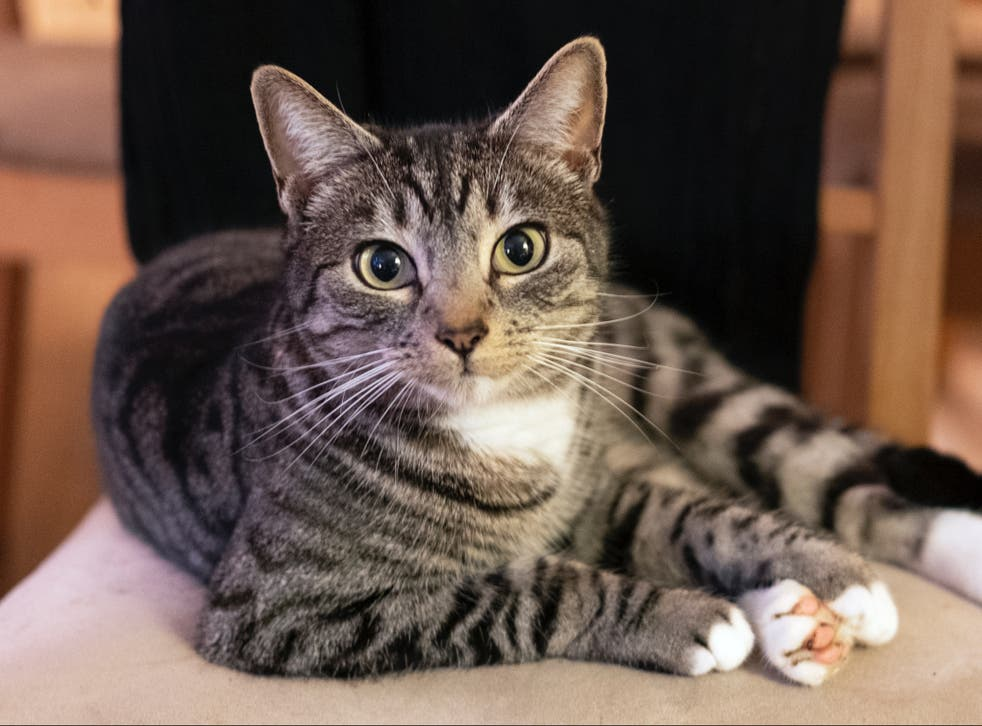
\includegraphics[width=0.5\linewidth]{cat}
			\caption{A random cat}
		\end{figure}	
	\end{center}
	
\end{document}
